%!TeX spellcheck = en-GB
\documentclass[12pt,a4paper]{report}

\usepackage[utf8]{inputenc}
\usepackage[english]{babel}
\usepackage{titling}
\usepackage{array}
\usepackage{amsmath}
\usepackage{graphicx}
\usepackage{epstopdf}
\usepackage{subfigure}
\usepackage{float}
\usepackage{placeins}
\usepackage{wrapfig}
\usepackage{diagbox}
\usepackage{hyperref}
\usepackage{pbox}
\usepackage{fancyhdr}
\usepackage[a4paper]{geometry}
\usepackage{header}
\usepackage[absolute,overlay]{textpos}
  \setlength{\TPHorizModule}{1mm}
  \setlength{\TPVertModule}{1mm}

\usepackage[show]{chato-notes} % change the "show" option to "hide" to remove all \todo and \note blocks


\geometry{hscale=0.8,vscale=0.8,centering}
\pagestyle{fancy}
\fancyhf{}
\fancyhead[L]{}
\fancyhead[R]{}
\cfoot{\thepage}
\setlength{\droptitle}{-6em}

\newcommand{\blap}[1]{\vbox to 0pt{#1\vss}}
\newcommand\AtUpperLeftCorner[3]{%
  \put(\LenToUnit{#1},\LenToUnit{\dimexpr\paperheight-#2}){\blap{#3}}%
}
\newcommand\AtUpperRightCorner[3]{%
  \put(\LenToUnit{\dimexpr\paperwidth-#1},\LenToUnit{\dimexpr\paperheight-#2}){\blap{\llap{#3}}}%
}

\newcommand\AtDownRightCorner[3]{%
  \put(\LenToUnit{\dimexpr\paperwidth-#1},\LenToUnit{#2}){\blap{\llap{#3}}}%
}

\newcommand{\HRule}{\rule{\linewidth}{0.5mm}}

\title{PROJ0011-1 Personal student project}
\subTitle{Integration of libopencm3 in FreeRTOS for STM32F4 and STM32F3 MCU}
\author{Pierre Nicolay}
\acYear{2018-2019}
\univ{University of Liège}
\date{\today}
\makeatletter

\begin{document}

\begin{titlepage}
  \begin{textblock}{30}(150,20)
      
\includegraphics[width=4cm]{Headers/ulg.png}
  \end{textblock}
  \begin{textblock}{30}(125,240)
      
\includegraphics[width=9.0cm]{Headers/facsa.png}
  \end{textblock}
  \hbox{
  \hspace*{0.2\textwidth}
  \rule{1pt}{\textheight}
  \hspace*{0.05\textwidth}
  \parbox[b]{0.75\textwidth}{ % P
  \begin{flushleft}
    {\noindent\Huge\bfseries \@title}\hspace*{0.2\textwidth}
    \\\HRule\\[2\baselineskip]
    {\Large \textsc{\@subTitle}}\\[4\baselineskip]
    {\large \textsc{\@author}}\\[2\baselineskip]
    {\large \textsc{\@univ: }}
    {\large \textsc{\@acYear}}\\[20\baselineskip]
    \@date
  \end{flushleft}
  \vspace*{0.05\textheight}
  \hspace*{0.3\textwidth}
  }}

\end{titlepage}

\tableofcontents

\newpage
\chapter{Introduction}
\label{ch:intro}
This project lies in the scope of the \emph{RoboCupSoccer competition} project. The reader that is already familiar with this competition can skip the introduction and pursue his reading at chapter \ref{ch:prob}.\newline
The Robocup competition is a international science and technology tournament created in 1997 \cite{robocupHistory}. The goal is to promote technology and advance the state-of-the-art in robotic and AI through a landmark project such as robot playing soccer. The ultimate goal however is ``By the middle of the 21st century, a team of fully autonomous humanoid robot soccer players shall win a soccer game, complying with the official rules of FIFA, against the winner of the most recent World Cup.'' \cite{RobocupObjective}.\newline
The university of liege wants to take part to the competition. Therefore we first need to build a robotic platform. The platform illustrated in figure \ref{fig:platform} is composed of joint and links. 

\begin{figure}[h]
  \begin{minipage}[c]{0.3\textwidth}
    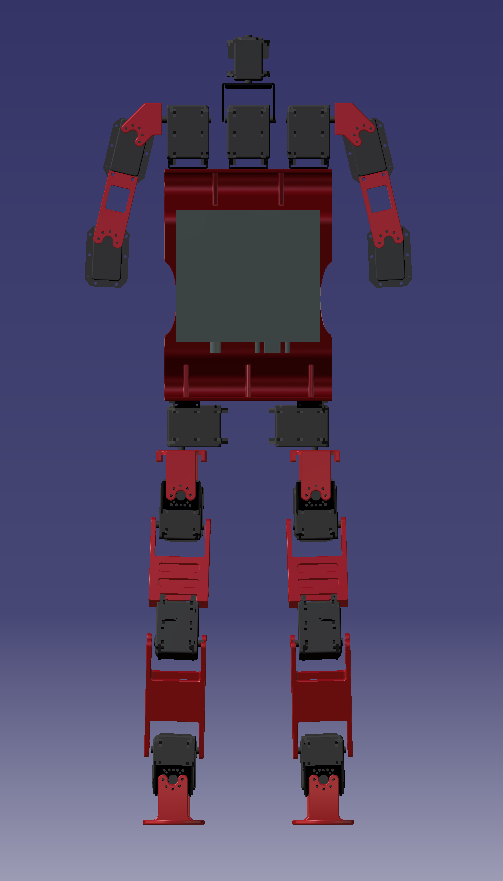
\includegraphics[width=\textwidth]{figs/platform.png}
  \end{minipage}\hfill
  \begin{minipage}[c]{0.6\textwidth}
    \caption{Image illustrating our platform. Each joint, in black, is a a servo motor (MX-28 \cite{MX28}) and each link, in red, is a 3D printed segment linking every joint together. The choice of this design is not discussed here.}
    \label{fig:platform}
  \end{minipage}
\end{figure}

The origin of this project comes out of the work of \cite{masterGL}. \cite{masterGL} proposed to change the internal electronic components of every servo in order to increase the control accuracy, easily implement a variety of handcrafted commands, implement more accurate sensors, enable communication through CAN bus and use of a more powerful microcontroller. The next logical part of the work is thus to add a software layer in order to use the new homemade board's feature.\newline
The goal of this project is to implement a software layer using a real time operating system (RTOS) as well as USB communication.\newline
This document's purpose is twofold, defining the problem and explaining the solution used to solve it as well as giving a documentation and a starting point for the \emph{uLiege robocup}'s team members in order to continue the project.\newline
In the next chapter we are going to define the problem we are facing and how it relates to the \emph{RoboCupSoccer competition} project. \newpage
\chapter{Problem Statement}
\label{ch:prob}
As mentioned previously, the goal of the project is mainly to use a a RTOS along with a mcu firmware. The mcus used on \cite{masterGL}'s board are part of the STM32F3 familly. In addition to this we also needed to handle the STM32F4 familly. The reason for this is that an other board is currently developped by \emph{uLiege robocup}'s team and the processor on this board will be of the STM32F4 type.\newline
Thus as we would like to communicate with different devices over a USB communication as well as drive the servomotors or even monitor every sensor we decided before beginning of the project to use a RTOS.\newline
The utility of the RTOS is multiple. First it give the programmer a comfortable programming work-frame for inter-process communication by providing tools such as semaphores, mutex, message Queue etc. In addition to this the RTOS provides a consistency concerning the execution time of each task.\newline
The RTOS chosen here is FreeRTOS. More details can be found in section~\ref{sec:freeRTOS}. We also needed a firmware to interact with the different functionalities of the mcu. The library chosen despite the existence of a vendor's one is \emph{Libopencm3} (section~\ref{sec:libopencm3}). 
\chapter{Libraries}
\section{Libopencm3}
\label{sec:libopencm3}
\section{FreeRTOS}
\label{sec:freeRTOS}
\chapter{Implementation details}
\section{USB}
\chapter{Documentation}
\chapter{Conclusion}
\section{troubleshooting}
\section{Future work}
\bibliography{references} 
\bibliographystyle{apalike}
\end{document}